\section{Hausdorffova dimenzija}
Hausdorffova dimenzija je najstarejši in matematično najosnovnejši poskus formalizacije dimenzije, ki velja tudi za fraktalne množice. Njena moč izhaja iz dejstva, da temelji na zunanji meri, kar omogoča natančno in splošno definicijo, ki velja za katerokoli podmnožico evklidskega prostora.

Čeprav je Hausdorffova dimenzija pogosto težko izračunljiva ali celo numerično nedostopna, ostaja ključno orodje pri razumevanju in klasifikaciji fraktalnih struktur. V nadaljevanju bomo spoznali njen formalni zapis ter nekaj osnovnih primerov in geometričnih lastnosti. Pokazali bomo tudi, da Hausdorffova dimenzija ustreza našemu intuitivnemu pojmu ">dobre"< dimenzije, ki smo jo iskali na začetku.

\subsection{Konstrukcija Hausdorffove mere}
Začnemo z konstrukcijo Hausdorffove mere, ki nam bo omogočila natančno definicijo Hausdorffove dimenzije in pripomogla k boljšemu razumevanju geometrije takšnih množic.

Najprej definiramo osnovna pojma.

\begin{definicija}
    Naj bo \((X, d)\) metrični prostor. Zunanja mera \(\mu^*\) na \(X\) je \emph{metrična zunanja mera}, če 
    \[\mu^*(A \cup B) = \mu^*(A) + \mu^*(B),\]
    za vsaki množici \(A, B \subseteq X\), za kateri velja \(d(A, B) > 0\).
\end{definicija}

Dokaz naslednje trditve lahko najdemo v \cite[stran 349]{f-ra}.
\begin{trditev}
    \label{m-zun-mera}
    Naj bo \((X, d)\) metrični prostor. Če je \(\mu^*\) metrična zunanja mera na \(X\), potem je njena zožitev na Borelovo \(\sigma\)-algebro \(\mu = \mu^*|_{\mc{B(X)}}\) mera na merljivem prostoru \((X, \mc{B}(X))\).
\end{trditev}

\begin{opomba}
    \(d(A, B) := \inf\setb{d(a, b)}{a \in A,\ b \in B}\).
\end{opomba}



Zdaj lahko definiramo Hausdorffovo zunanjo mero.
\begin{definicija}
    \label{def-haus-mera}
    Naj bo \((X, d)\) metrični prostor, \(p \geq 0\) in \(\delta > 0\). Za vsako podmnožico \(A \subseteq X\) definiramo 
    \[H^p_\delta(A) = \inf \setb{\sum_{i=1}^{\infty}(\diam A_i)^p}{A_i \subseteq X \land A \subseteq \un{i \in \N}{A_i} \land \diam A_i \leq \delta}.\]
    Ker se množica možnih pokritij množice \(A\) z zmanjševanjem \(\delta\) zmanjšuje, je funkcija \(H^p_\delta(A)\) naraščajoča glede na \(\delta\). Zato obstaja limita
    \[\mc{H}^p = \lim_{\delta \to 0} H_\delta^p(A)\]
    (končna ali neskončna), ki ji pravimo \emph{\(p\)-dimenzionalna Hausdorffova zunanja mera množice \(A\)}.

    Pokritje množice \(A\) z množicami premera največ \(\delta\) imenujemo \emph{\(\delta\)-pokritje množice \(A\)}.
\end{definicija}

\begin{opomba} \ 
    \begin{itemize}
        \item \(\diam A = \sup \setb{d(x, y)}{x, y \in A}\)
        \item \(\inf \emptyset = \infty\)
    \end{itemize}
\end{opomba}

\begin{opomba}
    \label{odp-zap-haus}
    V definiciji so \(A_i \subseteq X\) poljubne. Enak rezultat lahko dobimo, če se omejimo le na zaprte podmnožice, saj velja \(\diam A_i = \diam \overline{A_i}\), ali pa le na odprte podmnožice, saj lahko vsako množico \(A_i\) nadomestimo z množico \(U_i = \setb{x \in X}{d(x, A_i) < \frac{\varepsilon}{2^{i+1}}}\), ki ima premer kvečjemu \((\diam A_i) + \frac{\varepsilon}{2^i}\).

    Tukaj je \(d(x, A_i) = \inf \setb{d(x, a)}{a \in A_i}\).
\end{opomba}

Dokažemo osnovno lastnost \(\mc{H}_p\).
\begin{trditev}
    \label{haus-m-zun}
    Naj bo \((X, d)\) metrični prostor. \(\mc{H}_p\) je metrična zunanja mera.
\end{trditev}

\begin{proof}
    Po trditvi \ref{zun-mera} sledi, da je \(H^p_\delta\) zunanja mera na \(X\). Ker je limita monotona, sledi tudi, da je \(\mc{H}^p\) zunanja mera na \(X\).

    Naj bo \(A, B \subseteq X\) množici, za kateri velja \(d(A, B) > 0\). Izberimo tak \(\delta > 0\), da velja \(\delta < d(A, B)\). Naj bo \((C_i)_{i \in \N}\) družina podmnožic \(X\), ki je \(\delta\)-pokritje množice \(A \cup B\).
    Ker je \(\diam C_i < d(A, B)\) za vsak \(i \in \N\), nobena množica \(C_i\) ne seka hkrati množice \(A\) in množice \(B\). Razdelimo vsoto \(\sum_{i=1}^{\infty} (\diam C_i)^p\) na dva dela:
    \begin{itemize}
        \item \(\displaystyle \sum_{C_i \cap B = \emptyset} (\diam C_i)^p\) in
        \item \(\displaystyle \sum_{C_i \cap A = \emptyset} (\diam C_i)^p\).
    \end{itemize}
    Po definiciji infimuma velja 
    \[\sum_{i=1}^{\infty} (\diam C_i)^p \geq H^p_\delta(A) + H^p_\delta(B).\]
    Ker je bilo pokritje \((C_i)_{i \in \N}\) poljubno, sledi, da \(H^p_\delta(A) + H^p_\delta(B)\) spodnja meja za množico dolžin vseh \(\delta\)-pokritij množice \(A \cup B\). Zato po definiciji infimuma velja, da
    \[H_\delta^p(A \cup B) \geq H^p_\delta(A) + H^p_\delta(B).\]
    V limiti \(\delta \to 0\) dobimo:
    \[\mc{H}^p(A \cup B) \geq \mc{H}^p(A) + \mc{H}^p(B).\]

    Po definiciji zunanje mere, ki je subaditivna, pa velja tudi:
    \[H^p(A \cup B) \leq H^p(A) + H^p(B).\]
    Iz obeh neenakosti sledi enakost, torej \(\mc{H}^p\) zadošča pogoju metrike.
\end{proof}

Direktna posledica trditev \ref{m-zun-mera} in \ref{haus-m-zun} je
\begin{posledica}
    Naj bo \((X, d)\) metrični prostor. Zožitev Hausdorffove zunanje \(p\)-dimenzionalne mere na Borelovo \(\sigma\)-algebro 
    \[\mc{H}^p := \mc{H}^p|_{\mc{B}(X)}\]
    je mera na merljivem prostoru \((X,\mc{B}(X))\).
\end{posledica}

Brez dokaza navedemo še trditev, ki povezuje \(\mc{L}^n\) in \(\mc{H}^p\). Dokaz lahko najdemo v \cite[stran 351]{f-ra}.
\begin{trditev}
    \label{haus-leb}
    Naj bo \(n \in \N\). Obstaja konstanta \(c_n > 0\), da je \(c_n \mc{H}^n\) Lebesgueova mera na merljivem prostoru \((\R^n, \mc{B}(\R^n))\).
\end{trditev}

\begin{opomba}
    Konstanta \(c_n\) je volumen \(n\)-dimenzionalne krogle, tj. 
    \[c_n = \frac{\pi^{n/2}}{2^n \Gamma(\frac{n}{2} + 1)}.\]
\end{opomba}

V nadaljevanju bomo za metrični prostor \((X, d)\)  privzeli navaden evklidski prostor \((\R^n, d_2)\).

\subsection{Lastnosti Hausdorffove mere}
V tem razdelku bomo našteli in dokazali nekatere geometrijske lastnosti Hausdorffove mere, ki jih lahko prenesemo tudi na Hausdorffovo dimenzijo.

\subsubsection{Lastnosti skaliranja}
Lastnosti skaliranja so temeljne za razumevanje fraktalnih struktur, saj fraktali po svoji naravi izkazujejo samopodobnost. 

Naj bo \(P: \R^n \to \R^n\) \emph{podobnostna preslikava} s podobnostnim koeficientom \(\lambda > 0\), tj.\ preslikava, za katero velja
\[\all{x, y \in \R^n} |P(x) - P(y)| = c|x - y|.\]

\begin{opomba}
    Opazimo, da je vsaka podobnostna preslikava injektivna.
\end{opomba}

Intuitivno je jasno, da če raztegnemo daljico \(\lambda\)-krat, se njena dolžina poveča \(\lambda\)-krat, torej 
\[\mc{L}^1(P(A)) = \lambda\mc{L}^1(A),\]
če povečamo stranico kvadrata za faktor \(\lambda\), se njegova ploščina poveča za faktor \(\lambda^2\), torej 
\[\mc{L}^2(P(A)) = \lambda^2\mc{L}^2(A)\]
in tako naprej za višje dimenzije.

Naravno se pojavi vprašanje: ali podobna lastnost velja tudi za Hausdorffovo mero? Odgovor nam da naslednja trditev.

\begin{trditev}
    \label{skale}
    Naj bo \(P: \R^n \to \R^n\) podobnostna preslikava s podobnostnim koeficientom \(\lambda > 0\) in \(A \subseteq \R^n\), \(p \geq 0\). Tedaj velja:
    \[\mc{H}^p(P(A)) = \lambda^p \mc{H}^p(A).\]
\end{trditev}

\begin{proof}
    Naj bo \((A_i)_{i \in \N}\) \(\delta\)-pokritje množice \(A\). Tedaj je \((P(A_i))_{i \in \N}\) \(\lambda \delta\)-pokritje množice \(P(A)\), saj velja \(\diam(P(A_i)) = \lambda \diam(A_i)\). Torej:
    \[\sum_{i=1}^{\infty} (\diam P(A_i))^p = \sum_{i=1}^{\infty}(\lambda \diam A_i)^p = \lambda^p \sum_{i=1}^{\infty}(\diam A_i)^p.\]
    Po definiciji infimuma velja 
    \[H^p_{\lambda \delta} (P(A)) \leq \lambda^p \sum_{i=1}^{\infty}(\diam A_i)^p.\]
    Ker je \((A_i)_{i \in \N}\) bilo poljubno \(\delta\)-pokritje množice \(A\), dobimo:
    \[H^p_{\lambda \delta} (P(A)) \leq \lambda^p H^p_\delta(A).\]
    V limiti \(\delta \to 0\) dobimo:
    \[\mc{H}^p (P(A)) \leq \lambda^p \mc{H}^p(A).\]    
    
    Za obratno neenakost uporabimo enak argument na preslikavi \(P^{-1}\), ki je tudi podobnostna preslikava s koeficientom \(1/\lambda\), in na množici \(P(A)\). Dobimo:
    \[
        \mc{H}^p(A) \leq (1/\lambda)^p \mc{H}^p(P(A)) \lthen \mc{H}^p(P(A)) \geq \lambda^p \mc{H}^p(A).
    \]
    Skupaj s prvo neenakostjo sledi enakost.
\end{proof}

Navedemo eno pomembno posledico

\begin{posledica}
    Naj bo \(P: \R^n \to \R^n\) izometrija, tj.\ preslikava, za katero velja
    \[\all{x, y \in \R^n} |P(x) - P(y)| = |x - y|\]
    in \(A \subseteq \R^n\), \(p \geq 0\). Tedaj velja:
    \[\mc{H}^p(P(A)) = \mc{H}^p(A).\]    
\end{posledica}

Primeri izometrij so rotacije, translacije, zrcaljenja ipd. Posledica pove, da je \(\mc{H}^p\) invariantna glede na rotacije, translacije in zrcaljenja, kar je pričakovano.

\subsubsection{Transformacijske lastnosti}
Še en zanimiv razred preslikav so \emph{H\"oldorjeve preslikave} stopnje \(\alpha > 0\), t.j.\ preslikave \(f: X \subseteq \R^m \to \R^n\), za katere velja
\[\some{c > 0} \all{x, y \in X} |f(x) - f(y)| \leq c|x-y|^\alpha.\]
V posebnem primeru, ko je \(\alpha = 1\), pravimo, da je preslikava \(f\) \emph{Lipschitzeva}.

Z istim argumentom kot prej lahko dokažemo naslednjo trditev
\begin{trditev}
    \label{mera-hold}
    Naj bo \(X \subseteq \R^m\), \(A \subseteq X\) in \(f: X \to \R^n\) Höldorjeva preslikava stopnje \(\alpha > 0\) s konstanto \(c > 0\). Potem za vsak \(p \geq 0\) velja:
    \[\mathcal{H}^{p/\alpha}(f(A)) \leq c^{p/\alpha} \mathcal{H}^p(F).\]
\end{trditev}

Direktna posledica te trditve je 
\begin{posledica}
    Naj bo \(X \subseteq \R^m\), \(A \subseteq X\) in \(f: X \to \R^n\) Lipschitzeva preslikava s konstanto \(c > 0\). Potem za vsak \(p \geq 0\) velja:
    \[\mathcal{H}^{p}(f(A)) \leq c^p \mathcal{H}^p(A).\]
\end{posledica}

Zdaj smo pripravili vsa potrebna orodja za definicijo Hausdorffove dimenzije in za preučevanje njenih lastnosti.

\subsection{Hausdorffova dimenzija}
V tem razdelku bomo definirali Hausdorffovo dimenzijo množice.

Naj bo \(A \subseteq \R^n\). Definiramo funkcijo \(\mc{H}_A: [0, \infty) \to [0, \infty]\) s predpisom 
\[\mc{H}_A(p) = \mc{H}^p(A).\]
\begin{lema}
    Naj bo \(A \subseteq \R^n\). Če je \(\mathcal{H}^{p}(A) < \infty\), potem je \(\mathcal{H}^{t}(A) = 0\) za vse \(t > p\).
\end{lema}

\begin{proof}
    Naj bo \(\varepsilon > 0\). Naj bo \(\delta > 0\) in \((A_i)_{i \in \N}\) \(\delta\)-pokritje množice \(A\). Tedaj po definiciji infimuma velja
    \[H^{p + \varepsilon}_\delta(A) \leq \sum_{i=1}^{\infty} (\diam A_i)^{p + \varepsilon} = \sum_{i=1}^{\infty} (\diam A_i)^{p} (\diam A_i)^{\varepsilon} \leq \delta^{\varepsilon} \sum_{i=1}^{\infty} (\diam A_i)^{p},\]
    torej 
    \[H^{p + \varepsilon}_\delta(A) \leq \delta^{\varepsilon} \sum_{i=1}^{\infty} (\diam A_i)^{p}.\]
    Ker je \((A_i)_{i \in \N}\) bilo poljubno \(\delta\)-pokritje množice \(A\), dobimo:
    \[H^{p + \varepsilon}_\delta(A) \leq \delta^{\varepsilon} H^{p}_\delta(A).\]
    Ker je \(\mathcal{H}^{p}(A) < \infty\), v limiti \(\delta \to 0\) dobimo:
    \[\mc{H}^{p + \varepsilon}(A) \leq 0.\]
    Ker je \(\mc{H}_A\) nenegativna funkcija, sledi
    \[\mc{H}^{p + \varepsilon}(A) = 0\]
    za vsak \(\varepsilon > 0\).
\end{proof}

Sedaj si lahko ogledamo graf funkcije \(\mc{H}_A\)
\begin{center}
    \drawGraf
\end{center}
Vidimo, da obstaja kritična točka \(p_0 \in [0, \infty)\), pri kateri vrednost funkcije \(\mc{H}^p\) ">skoči"< z \(\infty\) na \(0\). Zato definiramo

\begin{definicija}
    \emph{Hausdorffova dimenzija množice \(A \subseteq \R^n\)} je 
    \[\dim_H A = \inf \setb{p \geq 0}{\mathcal{H}^{p}(A) = 0} = \sup \setb{p \geq 0}{\mathcal{H}^{p}(A) = \infty}.\]
\end{definicija}

\begin{opomba} \ 
    \begin{itemize}
        \item Po dogovoru je \(\sup \emptyset = 0\).
        \item Hausdorffova dimenzija je definirana za poljubno množico \(A \subseteq \R^n\), saj je opredeljena s pomočjo Hausdorffove zunanje mere.
    \end{itemize}    
\end{opomba}

\begin{opomba}
    Naj bo \(A \subseteq \R^n\). Potem velja:
        \[
            \mathcal{H}^{p}(A) = \begin{cases}
                \infty; &0 \leq p < \dim_H A \\ 
                0; &p > \dim_H A,
            \end{cases}
        \]        
        pri \(p = \dim_H A\) pa je \(\mc{H}^p(A)\) lahko katerakoli vrednost iz intervala \([0, \infty]\).
\end{opomba}

\begin{zgled}
    \label{dim-ball}
    Naj bo \(B^n = B(x, r) = \setb{y \in \R^n}{d(x, y) < r}\) odprta \(n\)-dim krogla s središčem v \(x \in \R^n\) in polmerom \(r > 0\). Po trditvi \ref{haus-leb} sledi, da velja
    \[\mc{H}^n(B^n) = \frac{1}{c_n} \mc{L}^n(B^n) = \frac{1}{c_n} \vol(B^n).\]
    Torej je 
    \[0 < \mc{H}^n(B^n) < \infty\]
    in 
    \[\dim_H B^n = n.\]
    Isti sklep velja tudi za zaprto kroglo \(\overline{B}^{\, n} \subseteq \R^n\), tj.
    \[\dim_H \overline{B}^{\, n} = n.\]
\end{zgled}

\begin{opomba}
    Obstajajo tudi druge ekvivalentne definicije Hausdorffove dimenzije, ki jih lahko najdemo v \cite{fk-fg}.
\end{opomba}

\subsection{Lastnosti Hausdorffove dimenzije}
Sedaj, ko smo definirali Hausdorffovo dimenzijo, lahko nadaljujemo z obravnavo njenih pomembnih geometričnih in topoloških lastnosti ter vpliva na strukturo množic.

\subsubsection{Splošne lastnosti}
Naslednja trditev je direktna posledica monotonosti Hausdorffove zunanje mere 

\begin{trditev}[Monotonost]
    \label{haus-monotonost}
    Hausdorffova dimenzija je monotona, tj.
    \[\all{A, B \subseteq \R^n} A \subseteq B \lthen \dim_H A \leq \dim_H B\]
\end{trditev}

\begin{trditev}[Števna stabilnost]
    \label{haus-stab}
    Naj bo \((A_i)_{i \in \N}\) družina podmnožic \(\R^n\). Tedaj velja 
    \[\dim_H \un{i \in \N}{A_i} = \sup \setb{\dim_H A_i}{i \in \N}.\]
\end{trditev}

\begin{proof}
    Označimo z \(s = \sup \setb{\dim_H A_i}{i \in \N}\). 
    
    Ker je \(A_i \subseteq \un{i \in \N}{A_i}\) za vsak \(i \in \N\) in je po trditvi \ref{haus-monotonost} Hausdorffova dimenzija monotona, sledi, da
    \[\dim_H F_i \leq \dim_H \un{i \in \N}{A_i}\]
    za vsak \(i \in \N\). Po definiciji supremuma velja:
    \[s \leq \dim_H \un{i \in \N}{A_i}.\]

    Naj bo \(\varepsilon > 0\). Po definiciji supremuma velja, da \(\dim_H A_i < s + \epsilon\) za vsak \(i \in \N\). Torej 
    \[\mc{H}^{s + \varepsilon}(A_i) = 0\]
    za vsak \(i \in \N\). Ker je Hausdorffova zunanja mera subaditivna, sledi, da
    \[\mc{H}^{s + \varepsilon}\left(\un{i \in \N}{A_i}\right) \leq \sum_{i=1}^{\infty} \mc{H}^{s + \varepsilon} (A_i) = 0.\]
    V limiti \(\varepsilon \to 0\) dobimo:
    \[\mc{H}^s\left(\un{i \in \N}{A_i}\right) \leq 0.\]
    Torej 
    \[\dim_H \un{i \in \N}{A_i} \leq s.\]    
    Skupaj s prvo neenakostjo sledi enakost.
\end{proof}

\begin{posledica}
    \label{dim-rn}
    Hausdorffova dimenzija \(\R^n\) je 
    \[\dim_H \R^n = n.\]
\end{posledica}

\begin{proof}
    Ker je prostor \(\R^n\) 2-števen, obstaja števno pokritje \((B^n_i)_{i \in \N}\) množice \(\R^n\) z odprtimi krogli. Po trditvi \ref{haus-stab} in zgledu \ref{dim-ball} sledi, da
    \[\dim_H \R^n \leq n.\]
    Ker pa velja \(B^n(0, 1) \subseteq \R^n\) in je po trditvi \ref{haus-monotonost} Hausdorffova dimenzija monotona, sledi tudi obratna neenakost:
    \[
        \dim_H \R^n \geq \dim_H B^n(0, 1) = n.
    \]
    Torej je \(\dim_H \R^n = n\).
\end{proof}

\begin{trditev}[Dimenzija števnih množic]
    Naj bo \(A \subseteq \R^n\). Če je \(A\) števna, potem 
    \[\dim_H A = 0.\]
\end{trditev}

\begin{proof}
    Ker je \(A\) števna množica, lahko jo zapišemo v obliki 
    \[A = \set{a_1, a_2, a_3, \ldots}.\]
    Definiramo \(A_i = \set{a_i}\) za vsak \(i \in \N\). Tedaj velja
    \[A = \un{i \in \N}{A_i}.\]
    Ker je \(0 < \mc{H}^0(A_i) = 1 < \infty\) sledi, da 
    \[\dim_H A_i = 0\]
    za vsak \(i \in \N\).
    Po trditvi \ref{haus-stab} velja
    \[\dim_H A = \dim_H \un{i \in \N}{A_i} = \sup \setb{\dim_H A_i}{i \in \N} = 0.\]
\end{proof}

\begin{zgled}
    Hausdorffova dimenzija \(\Q \subseteq \R\) je \(0\), saj je \(\Q\) števna množica. 
\end{zgled}

\begin{trditev}[Dimenzija odprtih množic]
    \label{haus-odp}
    Naj bo \(U \subseteq \R^n\). Če je \(U\) odprta in neprazna, potem 
    \[\dim_H U = n.\]
\end{trditev}

\begin{proof}
    Ker je \(U\) odprta in neprazna, vsebuje neko odprto \(n\)-dimenzionalno kroglo, po drugi strani pa je vsebovana v \(\R^n\). Trditev sledi.
\end{proof}

Ideje dokaza naslednje trditve lahko najdemo v \cite[stran 32]{fk-fg} in \cite[stran 351]{f-ra}.
\begin{trditev}[Dimenzija gladkih množic]
    Naj bo \(M \subseteq \R^n\). Če je \(M\) gladka (tj.\ \(C^\infty\)) podmnogoterost dimenzije \(m\), potem 
    \[\dim_H M = m.\]
    Posebej 
    \begin{itemize}
        \item Če je \(M\) gladka krivulja, potem \(\dim_H M = 1.\)
        \item Če je \(M\) gladka ploskev, potem \(\dim_H M = 2.\)
    \end{itemize}
\end{trditev}

\subsubsection{Transformacijske lastnosti}
Pri proučevanju Hausdorffove dimenzije se naravno zastavi vprašanje, kako se ta obnaša pri različnih transformacijah. Na primer: ali se dimenzija ohranja pri Lipschitzevih ali gladkih preslikavah? Takšna vprašanja so pomembna, saj nam transformacijske lastnosti pogosto omogočajo, da iz znane dimenzije neke množice sklepamo o dimenziji njene slike.

\begin{trditev}
    Naj bo \(X \subseteq \R^m\), \(A \subseteq X\) in \(f: X \to \R^n\) H\"oldorjeva preslikava stopnje \(\alpha > 0\) s konstanto \(c > 0\). Tedaj velja
    \[\dim_H f(A) \leq \frac{1}{\alpha} \dim_H A.\]
\end{trditev}

\begin{proof}
    Označimo z \(s:= \dim_H A\). Naj bo \(\varepsilon > 0\). Po trditvi \ref{mera-hold} velja
    \[\mc{H}^{(s +\varepsilon) / \alpha}(f(A)) \leq c^{(s +\varepsilon) / \alpha} \mc{H}^{s + \varepsilon}(A) = 0.\]
    V limiti \(\varepsilon \to 0\) dobimo
    \[\mc{H}^{s / \alpha}(f(A)) \leq 0,\]
    torej
    \[\dim_H f(A) \leq \frac{1}{\alpha} \dim_H A.\]
\end{proof}

V primeru Lipschitzevih preslikav (kjer je \(\alpha = 1\)) dobimo naslednjo pomembno posledico.

\begin{posledica}
    \label{dim-lips}
    Naj bo \(X \subseteq \R^m\), \(A \subseteq X\) in \(f: X \to \R^n\) Lipschitzeva preslikava s konstanto \(c > 0\). Tedaj velja
    \[\dim_H f(A) \leq \dim_H A.\]
\end{posledica}

Poseben primer Lipschitzevih preslikav so bi-Lipschitzeve preslikave. V tem primeru se Hausdorffova dimenzija ne spremeni -- to je povsem pričakovano, saj bi-Lipschitzeva preslikava ">niti ne sesuje"< niti ">neskončno ne raztegne"< razdalj: ohrani geometrijske razdalje ">v razumnem obsegu"<.

\begin{izrek}
    Naj bo \(X \subseteq \R^m\), \(A \subseteq X\) in \(f: X \to \R^n\) bi-Lipschitzeva preslikava, tj.\ preslikava \(f: X \to \R^n\), za katero velja:
    \[\some{c_1, c_2 > 0} \all{x, y \in X} c_1|x-y| \leq |f(x) - f(y)| \leq c_2|x-y|.\]
    Tedaj velja
    \[\dim_H f(A) = \dim_H A.\]
\end{izrek}

\begin{proof}
    Ker je \(f\) injektivna, je njena zožitev \(f: X \to f(X)\) bijektivna z Lipschitzevim inverzom \(f^{-1}: f(X) \to X\) s konstanto \(1 / c_1\). Po posledici~\ref{dim-lips} imamo
    \[\dim_H f(A) \leq \dim_H A\]
    in 
    \[\dim_H A = \dim_H f^{-1}f(A) \leq \dim_H f(A).\]
    Skupaj s prvo neenakostjo sledi enakost.
\end{proof}

Izrek pove, da je Hausdorffova dimenzija invariantna glede na bi-Lipschit\-zeve preslikave. To pomeni, da so bi-Lipschitzeve transformacije ">dimenzijsko ohranjajoče"<. Če imata dve množici različno Hausdorffovo dimenzijo, potem med njima ne more obstajati bi-Lipschitzeva preslikava.

\begin{opomba}
    Podoben princip poznamo tudi iz topologije: če imata prostora različni topološki invarianti (npr.\ različno število luknj), potem med njima ne more obstajati homeomorfizem. Hausdorffova dimenzija je torej v tem smislu geometrična in varna pred ">zmerno deformacijo"<.
\end{opomba}

\subsubsection{Topološke lastnosti}
Hausdorffova dimenzija ima tudi zanimivo povezavo s topologijo. Naslednji rezultat kaže, da dovolj ">majhne"< množice (v smislu dimenzije) ne morejo biti povezane.

\begin{trditev}
    \label{povezanost}
    Naj bo \(A \subseteq \R^n\). Če je \(\dim_H A < 1\), potem je \(A\) popolnoma nepovezana, torej so njene komponente za povezanost enojci.
\end{trditev}

\begin{proof}
    Naj bosta \(x, y \in A, \ x \neq y\). Definiramo preslikavo \(f: A \to [0, \infty)\) s predpisom
    \[f(z) = |z-x|.\]
    Preslikava \(f\) je Lipschitzeva, saj za vse \(z, w \in A\) velja:
    \[
        |f(z) - f(w)| = ||z - x| - |w - x|| \leq |z - w|.
    \]
    Po posledici~\ref{dim-lips} sledi:
    \[
        \dim_H f(A) \leq \dim_H A < 1.
    \]
    Znano pa je (trditev \ref{haus-odp}), da vsaka neprazna odprta množica v \(\R\) ima Hausdorffovo dimenzijo \(1\), zato \(f(A)\) ne vsebuje nobene neprazne odprte podmnožice, saj je \(\dim_H\) monotona. Torej je \(\comp{f(A)}\) gosta v \(\R\).

    Ker je \(0 < f(y)\), obstaja \(r \in (0, f(y))\), da \(r \notin f(A)\). Definiramo množici:
    \[
        U := \{ z \in A \mid f(z) < r \}, \quad V := \{ z \in A \mid f(z) > r \}.
    \]
    Množici \(U\) in \(V\) sta odprti v podprostoru \(A\) (kot prasliki odprtih množic v \([0, \infty)\), disjunktni in pokrivata cel \(A\), saj \(r \notin f(A)\). Poleg tega velja \(x \in U\) (ker je \(f(x) = 0 < r\)) in \(y \in V\) (ker je \(f(y) > r\)). Torej \(x\) in \(y\) ležita v različnih komponentah za povezanost množice \(A\).

    Ker sta bili \(x\) in \(y\) poljubno izbrani različni točki, sledi, da je vsaka komponenta množice \(A\) enojec.
\end{proof}

Ta rezultat pokaže, kako lahko Hausdorffova dimenzija vpliva na topološke lastnosti množic. Če je dimenzija strogo manjša od \(1\), je množica tako »tanka«, da je ni mogoče povezati niti z najkrajšo zvezno potjo. 

\subsection{Primeri računanja Hausdorffove dimenzije}
V tem razdelku bomo obravnavali primere izračuna Hausdorffove dimenzije za bolj zapletene množice. Običajno postopamo tako, da z geometrijskim premislekom podamo spodnjo in zgornjo oceno za dimenzijo ter upamo, da se ti meji ujemata. V tem primeru lahko sklepamo, da smo našli točno dimenzijo.

% \subsubsection{Cantorjev prah}
% Izračunamo dimenzijo Cantorjevega praha (slika \ref{fig:cantor-dust}). Cantorjev prah je fraktal, ki ga dobimo na naslednji način:

% \begin{enumerate}
%     \item Naj bo \(E_0\) kvadrat s stranico dolžine \(1\).
%     \item Kvadrat \(E_0\) razdelimo na \(16\) enakih manjših kvadratov tako, da vsako stranico razdelimo na 4 enake dele.
%     \item V vsaki vrstici izberemo en kvadrat (po določenem pravilu), ostale kvadrate pa odstranimo. Tako dobimo množico \(E_1\), ki je unija 4 kvadratov z dolžino stranice \(4^{-1}\).
%     \item Recimo, da imamo množico \(E_n\), ki jo sestavlja \(4^n\) kvadratov z dolžino stranice \(4^{-n}\). Za generacijo \(E_{n+1}\) vsak kvadrat iz \(E_n\) razdelimo na 16 manjših kvadratov in iz vsake vrstice izberemo po en kvadrat po istem pravilu kot prej, ostale odstranimo.
%     \item Postopek nadaljujemo induktivno.
% \end{enumerate}

% \begin{figure}[ht]
%     \centering
%     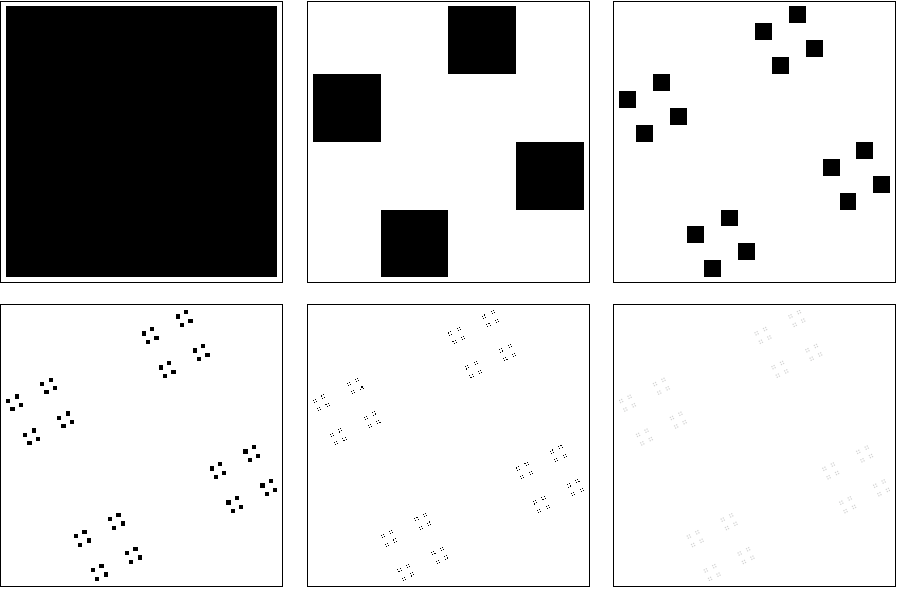
\includegraphics[width=\textwidth]{img/cantor_dust.pdf}
%     \caption{Cantorjev prah (Cantor dust).}
%     \label{fig:cantor-dust}
% \end{figure}

% \begin{definicija}
%     \emph{Cantorjev prah} je množica
%     \[
%     E = \bigcap_{i \in \N_0} E_i.
%     \]
% \end{definicija}

% \begin{trditev}
%     Hausdorffova dimenzija Cantorjeva praha je
%     \[\dim_H E = 1.\]
% \end{trditev}

% \begin{proof}
%     Naj bo \(E_k\) \(k\)-ta generacija konstrukcije. Tedaj \(E_k\) vsebuje \(4^k\) kvadratov s stranico \(4^{-k}\) in premerom največ \(4^{-k} \sqrt{2}\).

%     Naj bo \(\delta > 0\). Potem obstaja \(k \in \N\), da velja \(4^{-k} \sqrt{2} \leq \delta\). Kvadrati iz \(E_k\) tvorijo \(\delta\)-pokritje množice \(E\), zato dobimo oceno
%     \[H^1_\delta \leq 4^k 4^{-k}\sqrt{2} = \sqrt{2}.\]
%     V limiti \(\delta \to 0\) sledi
%     \[\mc{H}^1(E) \leq \sqrt{2},\]
%     torej 
%     \[\dim_H E \leq 1.\]

%     Naj bo zdaj \(\pi_x: E \to [0,1]\) projekcija na \(x\)-os, podana s predpisom
%     \[
%         \pi_x(x, y) = x.
%     \]
%     Po konstrukciji množice \(E\) je \(\pi_x(E) = [0,1]\), torej je preslikava surjektivna. Poleg tega je \(\pi_x\) Lipschitzeva, saj
%     \begin{multline*}
%         |(x_1, y_1) - (x_2, y_2)| = |(x_1 - x_2, y_1 - y_2)| = \sqrt{(x_1 - x_2)^2 + (y_1 - y_2)^2} \geq \\ \sqrt{(x_1 - x_2)^2} = |x_1 - x_2| = |\pi_x(x_1, y_1) - \pi_x(x_2, y_2)|.
%     \end{multline*}
%     Po posledici \ref{dim-lips} sledi
%     \[1 = \dim_H \pi_x (E) \leq \dim_H E.\]
%     Skupaj s prvo neenakostjo sledi enakost.
% \end{proof}

\subsubsection{Cantorjeva množica}
Izračunamo dimenzijo Cantorjeve množice (slika \ref{fig:cantor-set}).

\begin{trditev}
    Hausdorffova dimenzija Cantorjeve množice je
    \[\dim_H C = \log_3 2.\]
\end{trditev}

\begin{proof}    
    Naj bo \(C_k\) \(k\)-ta generacija konstrukcije. Tedaj \(C_k\) vsebuje \(2^k\) intervalov dolžine \(3^{-k}\). Označimo \(s = \log_3 2\).

    Naj bo \(\delta > 0\). Potem obstaja \(k \in \N\), da velja \(3^{-k} \leq \delta\). Intervali iz \(C_k\) tvorijo \(\delta\)-pokritje množice \(C\), zato dobimo oceno
    \[H^s_\delta(C) \leq 2^k \cdot 3^{-ks} = 1.\]
    V limiti \(\delta \to 0\) sledi
    \[\mc{H}^s(C) \leq 1,\]
    torej 
    \[\dim_H C \leq s.\]

    Naj bo \(\delta > 0\). Naj bo \((U_i)_{i \in \N}\) poljubno \(\delta\)-pokritje množice \(C\). Po opombi~\ref{odp-zap-haus} lahko brez škode za splošnost predpostavimo, da so \(U_i\) odprte množice. Ker je \(C\) kompaktna (tj.\ omejena in zaprta), obstaja končno podpokritje 
    \[U_1, U_2, \ldots, U_N.\]
    Za vsak \(i \in \set{1, 2, \ldots, N}\) izberimo \(k \in \N\), da velja
    \[3^{-(k + 1)} \leq \diam U_i < 3^{-k}. \tag{1}\]
    Tedaj \(U_i\) seka kvečjemu en interval v generaciji \(C_k\), saj je razdalja med dvema sosednjima intervaloma v tej generaciji vsaj \(3^{-k}\).

    Če je \(j \geq k\), potem po konstrukciji Cantorjeve množice \(U_i\) lahko seka kvečjemu \(2^{j - k}\) intervalov generacije \(C_j\), saj se pri vsakem koraku \(C_n \to C_{n+1}\) vsak interval razdeli na dva.

    Iz (1) sledi
    \[2^{j - k} = 2^k \cdot 3^{-sk} = 2^j \cdot 3^s \cdot (3^{-(k+1)})^s \leq 2^j \cdot 3^s \cdot (\diam U_i)^s. \tag{2}\]
    Torej vsak \(U_i\) seka kvečjemu \(2^j \cdot 3^s \cdot (\diam U_i)^s\) intervalov generacije \(C_j\).

    Če izberemo dovolj velik \(j \in \N\), da za vsak \(i \in \set{1, 2, \ldots, N}\) velja
    \[3^{-(j+1)} \leq \diam U_i,\]
    potem pokritje \((U_i)_{i \in \N}\) seka vsak izmed \(2^j\) intervalov v generaciji \(C_j\). S preštevanjem teh intervalov in uporabo (2) dobimo oceno
    \[2^j \leq \sum_{i=1}^{N} 2^j \cdot 3^s \cdot (\diam U_i)^s,\]
    od koder sledi
    \[\frac{1}{3^s} \leq \sum_{i=1}^{N} (\diam U_i)^s \leq \sum_{i=1}^{\infty} (\diam U_i)^s.\]
    Ker je bilo pokritje \((U_i)_{i \in \N}\) poljubno, po definiciji infimuma sledi, da 
    \[\frac{1}{3^s} \leq H^s_\delta(C).\]
    V limiti \(\delta \to 0\) dobimo
    \[\mc{H}^s(C) \geq \frac{1}{3^s} = \frac{1}{2},\]
    torej 
    \[\dim_H C \geq s.\]

    Skupaj s prvo neenakostjo sledi enakost.
\end{proof}

Iz zgornjega računa in topoloških lastnosti Hausdorffove dimenzije sledi naslednje:
\begin{posledica}
    Cantorjeva množica \(C\) je popolnoma nepovezana.
\end{posledica}

\begin{opomba}
    Iz zgornjega računa vidimo, da ima Cantorjeva množica res neničelno \(\log_3 2\)-dimenzionalno mero (oz.\ velikost). Z natančnejšo spodnjo oceno se lahko pokaže, da velja
    \[
        \mc{H}^s(C) = 1.
    \]
    Tak natančen izračun najdemo v \cite{pearse2014}.

    Če si predstavljamo, da ima Cantorjeva množica maso 1 kg, potem zaradi lastnosti skaliranja Hausdorffove mere (trditev \ref{skale}), če bi množico raztegnili dvakrat -- torej začeli z intervalom \([0,2]\) namesto \([0,1]\) — bi se njena masa povečala za faktor \(2^{\log_3 2}\) in bi bila približno enaka \(1,59\) kg.
\end{opomba}

Vidimo, da je izračun Hausdorffove dimenzije pogosto izredno zahteven, celo za preproste množice. Najprej je treba s pomočjo geometrijskih opažanj, simetrije ali samopodobnosti uganiti pravo vrednost dimenzije, nato pa to vrednost še dokazati. Ta postopek zahteva natančno analizo in pogosto precej tehničnega znanja.

Zato se naravno pojavi vprašanje: katere alternativne definicije dimenzije so nam na voljo?
